\documentclass{article}
\usepackage{hyperref}
\usepackage{graphicx}
\begin{document}
\title{Measuring Icebergs: Different Estimates of COVID-19 Cases in Portugal and Spain}
\author{$@$CoronaSurveys Team \\ \texttt{https://github.com/GCGImdea/coronasurveys}\\(draft in progress, not peer-reviewed)}
\maketitle
\section{Introduction}

During the current coronavirus pandemics, monitoring the evolution of COVID-19 cases is an important component for awareness and to inform policy decisions. 
Official numbers of laboratory confirmed cases are periodically issued by each country's health authority, for Portugal see \url{https://covid19.min-saude.pt}. 

Typically, along an outbreak testing eligibility criteria can evolve and the number of available tests also. Under these circumstances the evolution of official laboratory confirmed cases might not represent the total number of cases (see \url{https://www.nature.com/articles/d41586-020-00760-8}).  

This motivates looking at other probing techniques and try to bring in more information about the potential numbers. Actually the true numbers might only be known in the future once serological surveys are done (as done in prior outbreaks \url{https://journals.plos.org/plosone/article?id=10.1371/journal.pone.0050770}.

Bellow we consider two approaches: (a) Inferring current cases from the case fatality series; (b) Using crowdsourcing with anonymous surveys of indirect information.  

\section{Delay-adjusted case fatality ratio}

If we look at the current number of fatalities and divide it with the current number of confirmed cases, we obtain a naive case fatality ratio (CFR). However this metric does not take into account the number of cases with known outcomes, since recent cases will still evolve into fatalities and recoveries. By estimating the true number of cases with known outcomes, it is possible to obtain a corrected case fatality ratio (cCFR), as in \url{https://journals.plos.org/plosone/article?id=10.1371/journal.pone.0006852}, that takes into account the average delay from symptoms to death.  

Since the corrected denominator (cases with known outcomes) is reduced, the cCFR is higher than the naive CFR during a growing outbreak. A high cCFR is typically an indicator of lack of coverage in laboratory testing. If we assume, in general, that the disease will have similar case fatality rates in different countries it is possible use the known fatality ratio from Wuhan, China, currently at $1.38\%$
to compare with the obtained cCFR and estimate the percentage of coverage in different countries. This is done in \url{https://cmmid.github.io/topics/covid19/severity/global_cfr_estimates.html} and, for instance, the projected coverage in Portugal and Spain is $19\%$ and $4.7\%$. These values can in turn be used to correct the number of reported confirmed cases in each country and estimate the likely true number of cases, thus probing the iceberg that lurks under water.

Another technique, based on the same corrections for delay, but using an overall gross value for estimating the true cases from the mortality rate is simply obtained by multiplying the cumulative mortality by 400. See \url{https://www.nature.com/articles/d41586-020-00760-8}. We will use both techniques for estimation in each country.

\section{Crowdsourcing with anonymous surveys}

The $@$CoronaSurveys effort is based on crowdsourcing data in a way that avoids querying the users about their particular health status and identity. Participants can answer for a whole country or a region within a country. They answer two simple questions: 

\begin{itemize}
\item How many people do you know in this geographical area? (Please, consider only people whose current health status you likely know.)
\item As far as you know, how many of the above have symptoms compatible with COVID-19 (or were diagnosed with the disease)?
\end{itemize}

By not asking any personal information we aim to protect users privacy and having just two questions aims to make the process easy and repeatable with few effort from respondents. However the lack of more detailed information also makes the estimation process more challenging. We also do not control the spread of the survey and the adequate coverage of regions, age groups and other parameters.
Given this limitations, we can still obtain a gross estimate and see how it compares with other techniques. The obvious advantage is that this approach is very simple to deploy and can give very timely results. 

Surveyed responses are cleaned by identifying and removing outliers, in terms of the range of persons that the respondent declares to know (we remove entries outside 1.5 times the interquartile range above the upper quartile), and the ratio of symptomatic people reported (we remove entries above $30\%$ of reporting). We aim to survey the general population, that is not in particular high contact with symptomatic cases. Once the data is processed we obtain an estimate of the percentage of cases in the population that is known to the respondents and can naively extrapolate this ratio to the whole country population. 


Our initial surveys were done on Twitter and did not ask for how many people are known to the respondents. For those the reach was set to 150, which is the Dunbar number, characterizing the expected number of persons with whom one can maintain stable social relationships \url{https://en.wikipedia.org/wiki/Dunbar%27s_number}. 

In the following sections we show some results for the two countries. 

\section{The Portuguese data}

Portuguese data on fatality and confirmed cases was obtained in \url{https://github.com/dssg-pt/covid19pt-data}, a public repository that helps disseminated the official DGS daily data.

\begin{figure}
\begin{center}
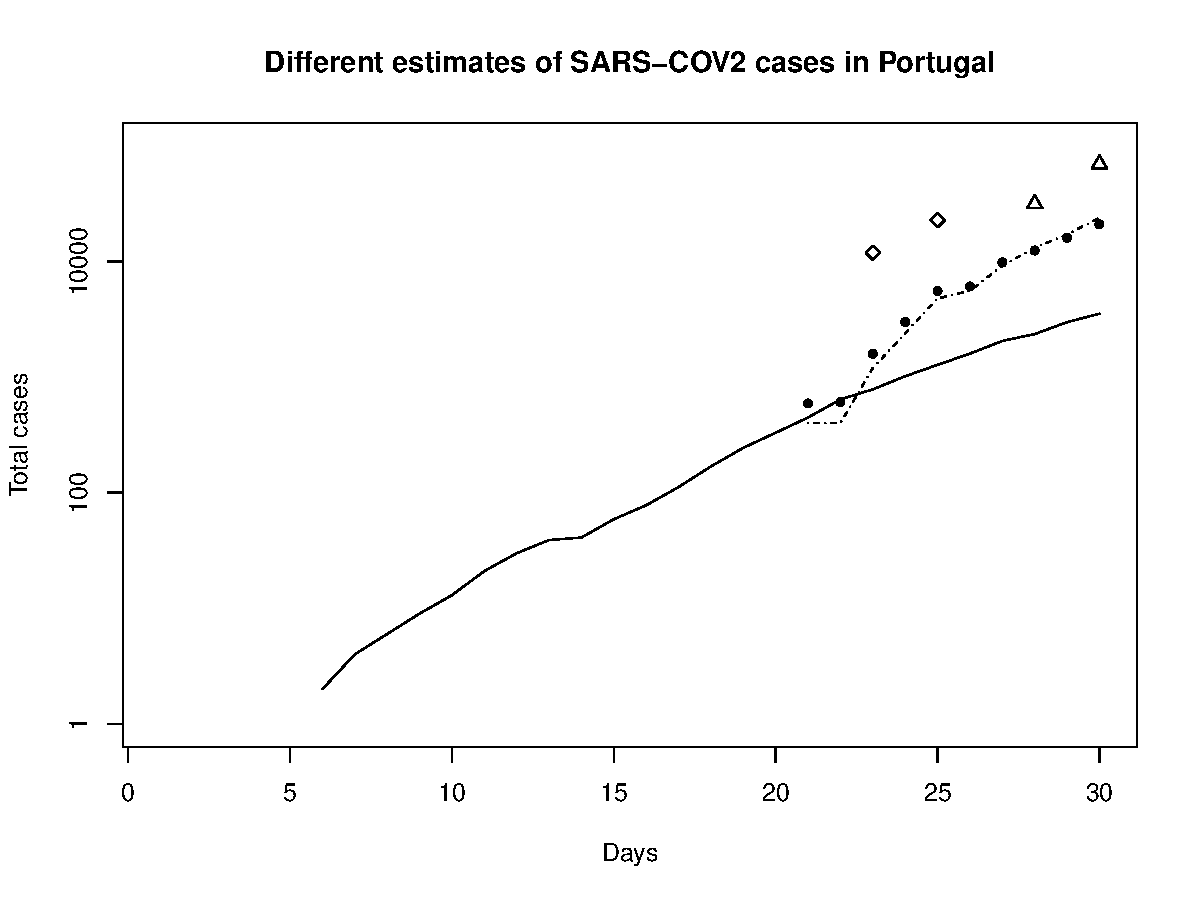
\includegraphics[width=.9\linewidth]{EstPTMar26.pdf}
\end{center}
\caption{Case estimates for Portugal, March 26th 2020.}
\label{pt}
\end{figure}

In Figure~\ref{pt} the solid line represents how many confirmed cases have been reported. The dashed line is the fatality number multiplied by 400, while the solid dots $\bullet$ indicate the more precise estimate from the corrected case fatality rates and compensating for the estimated coverage of testing. Finally, the diamond $\diamond$ represents our estimates from the two initial Twitter surveys and the triangles $\triangle$ the results from the subsequent two surveys via Google Forms. 

As we can see the anonymous surveys, by $@$CoronaSurveys, tend to estimate more cases, likely over-estimating, but still follow the overall tendency and surprisingly might be closer to the order of magnitude of the true numbers than the official reports. 
%On March 26, in Portugal, the official cases were 4268, the cCFR was reporting 25662 and our survey indicated 69839.  

\section{The Spanish data}

Spanish data was obtained from the European Center for Disease Control in \url{https://www.ecdc.europa.eu/}, with public information about COVID-19 cases across the World. 

\begin{figure}
\begin{center}
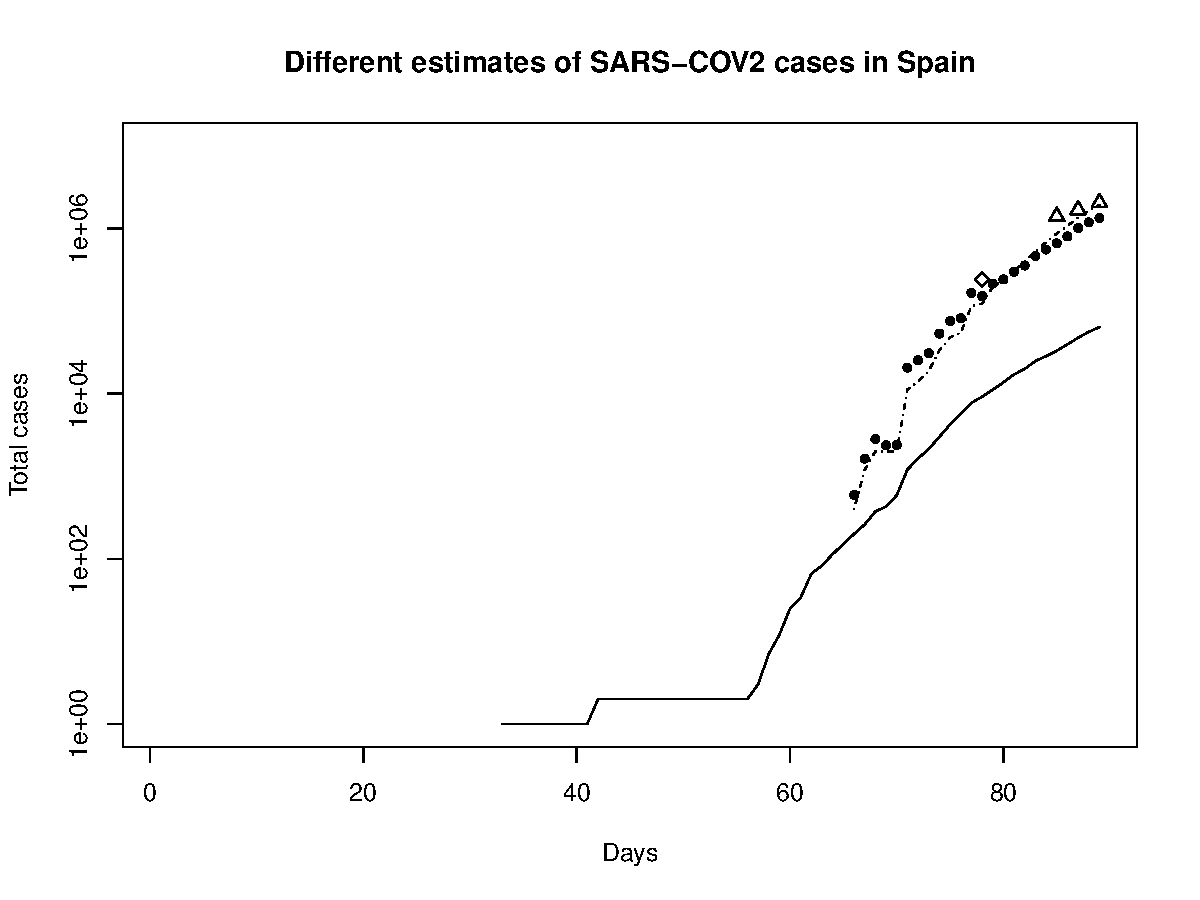
\includegraphics[width=.9\linewidth]{EstSPMar28.pdf}
\end{center}
\caption{Case estimates for Spain, March 28th 2020.}
\label{sp}
\end{figure}

For the Spanish case, see Figure~\ref{sp}, there is a even wider gap between cases predicted by fatality numbers and the reported cases. We include data points from one twitter survey and three subsequent Google Forms surveys. Surprisingly, the results from $@$CoronaSurveys are very close to the fatality based estimators, while providing still slightly higher estimates. 

\section{Discussion}

In this first report we draw attention to the limitations of relying only on confirmed cases to measure the true size of a growing pandemic. From existing data it is possible to derive other measures, and, surprisingly, it is also possible to do simple surveying approaches that, while simple and maybe crude, are clearly non invasive of privacy, and still get meaningful data. In particular  $@$CoronaSurveys can be relevant in countries with a decent digital infrastructure but lacking in laboratory resources. When measuring icebergs,  there are many strategies. 

\end{document}
